\documentclass[10pt,twocolumn,journal]{IEEEtran}
% XeLaTeX: all fonts are resolved from the local installation.
\usepackage{fontspec}
\defaultfontfeatures{Ligatures=TeX}
\setmainfont[
  BoldFont=TeXGyreTermes-Bold,
  ItalicFont=TeXGyreTermes-Italic,
  BoldItalicFont=TeXGyreTermes-BoldItalic,
  SmallCapsFont=TeXGyreTermes-Regular,
  SmallCapsFeatures={Letters=SmallCaps}
]{TeXGyreTermes-Regular}
\IfFontExistsTF{Arial}{\setsansfont{Arial}}{\setsansfont{Liberation Sans}}
\setmonofont{TeXGyreCursor-Regular}

\usepackage[margin=1in,bottom=1in]{geometry}
% Normal line spacing; content hierarchy provides the space savings.
\setlength{\textfloatsep}{10pt plus 2pt minus 2pt}
\setlength{\dbltextfloatsep}{10pt plus 2pt minus 2pt}
\setlength{\floatsep}{7pt plus 2pt minus 2pt}
\setlength{\abovecaptionskip}{4pt}
\usepackage{amsmath,amssymb}
\usepackage{booktabs,array}
\usepackage{graphicx}
\usepackage{xr-hyper}
\usepackage[hidelinks]{hyperref}
\usepackage{fancyhdr}
\graphicspath{{figures/}}
\setcounter{equation}{13}
\setcounter{table}{4}
\setcounter{figure}{4}
\setlength{\emergencystretch}{2em}
\renewcommand{\topfraction}{0.95}
\renewcommand{\dbltopfraction}{0.95}
\renewcommand{\textfraction}{0.05}
\renewcommand{\floatpagefraction}{0.85}
\renewcommand{\dblfloatpagefraction}{0.85}
\setcounter{topnumber}{3}
\setcounter{dbltopnumber}{3}
\pagestyle{fancy}
\fancyhf{}
\fancyhead[L]{\scriptsize BELOW ZERO --- SUPPLEMENTARY MATERIAL}
\fancyhead[R]{\scriptsize\thepage}
\renewcommand{\headrulewidth}{0pt}
\externaldocument{main}[main.pdf]
\makeatletter\setlength{\@fptop}{0pt}\setlength{\@fpsep}{16pt}\setlength{\@fpbot}{0pt plus 1fil}\makeatother
\newcommand{\BZAuthorBlockEN}{Yaogeng Jiang\\Independent Researcher\\\href{mailto:y.g.jiang@sjtu.edu.cn}{y.g.jiang@sjtu.edu.cn}}
\newcommand{\BZAuthorBlockZH}{姜尧耕\\独立研究者\\\href{mailto:y.g.jiang@sjtu.edu.cn}{y.g.jiang@sjtu.edu.cn}}
\newcommand{\BZPDFAuthors}{Yaogeng Jiang}

\hypersetup{pdfauthor={\BZPDFAuthors}}
\begin{document}
\title{Below Zero: Supplementary Material}
\author{\BZAuthorBlockEN}
\maketitle
\thispagestyle{fancy}

This supplement provides implementation details, regional analyses, calibration, and development-set controls. Numbering continues from the main text; full-precision scores and source-image identifiers are included with the accompanying data.

\section{Units, Conditioning, and the Meaning of a Sample}
\subsection{Signal Versus Readout}
The network output $s\geq0$ is an expected signal in DN; the corresponding electron mean is $s/g$. With $N\sim\operatorname{Poisson}(s/g)$, the simulator's integer path is
\begin{equation}
\begin{aligned}
A&=\min\{16383,\lfloor512+gN+\epsilon+b+1/2\rfloor\},\\
V&=A-512.
\end{aligned}
\end{equation}
All admitted simulated samples satisfy the physical lower ADC bound. Four-phase offsets are independently uniform over $[-0.25,0.25]$ DN and enter the estimator and decoder as known conditions.

A zero observation implies $V_i\leq0$. Under independent sensor noise, neighboring observations inform the latent signal; the conditional law at the estimated signal supplies the missing readout distribution.

Let $m=\mathbb E[V\mid Y,s]$ and $v=\operatorname{Var}(V\mid Y,s)$ at a censored pixel. For an independent draw $V'$ from the same conditional law,
\begin{align}
\mathbb E[(V-m)^2\mid Y,s]&=v,\\
\mathbb E[(V-V')^2\mid Y,s]&=2v.
\end{align}
A squared-error criterion therefore favors the conditional mean, which suppresses variation, over a statistically correct draw. This motivates the distribution scores used in the main comparison.

\subsection{Excess Scores and the Known-Signal Reference}
For the known-signal conditional law $p_i^\star$ and a prediction $q_i$ on a common discrete support,
\begin{equation}
\mathbb E_{V\sim p_i^\star}[-\log q_i(V)]-H(p_i^\star)=D_{\mathrm{KL}}(p_i^\star\|q_i).
\end{equation}
For the ranked probability score, expansion of the squares gives
\begin{equation}
\begin{split}
&\mathbb E_{V\sim p_i^\star}[\operatorname{CRPS}(q_i,V)-\operatorname{CRPS}(p_i^\star,V)]\\
&\qquad=\Delta\sum_k\left(F_{q_i}(k)-F_{p_i^\star}(k)\right)^2.
\end{split}
\end{equation}
These identities separate conditional uncertainty from distribution-estimation error. The known-signal law has zero self-divergence and cumulative discrepancy, while its realized NLL remains nonzero.

For a negative label, zero fill has ranked score $|V|$ and infinite NLL. The main table reports these values directly.

\section{Network, Data, and Training Details}
\subsection{Network Architecture}
We pack the Bayer phases as $[R,G_1,G_2,B]$ and provide 16 input channels: four $\operatorname{asinh}(Y/4)$ measurements, four zero-candidate indicators, four broadcast offset maps, a validity mask, and constant maps for $g$, $\sigma_r$, and a reserved zero. The validity mask distinguishes padded pixels from measured zeros. The known offsets enter both the estimator and the PG decoder.

Table~\ref{tab:architecture} gives the NAF-style architecture. Each normalization operates across channels at one spatial position, using FP32 arithmetic and $\epsilon=10^{-6}$. SimpleGate multiplies two channel halves, and learned residual scales are initialized to zero.

\begin{table}[t]
\centering
\caption{N0 architecture in packed CFA coordinates.}
\label{tab:architecture}
\footnotesize
\setlength{\tabcolsep}{3pt}
\begin{tabular}{@{}lccc@{}}
\toprule
Stage & Width & Blocks & Spatial scale\\
\midrule
Input stem & 32 & --- & 1\\
Encoder 1 & 32 & 2 & 1\\
Encoder 2 & 64 & 2 & 1/2\\
Encoder 3 & 128 & 4 & 1/4\\
Encoder 4 & 256 & 4 & 1/8\\
Bottleneck & 512 & 4 & 1/16\\
Decoder 1--4 & 256/128/64/32 & 2 each & 1/8 to 1\\
Signal head & 4 & --- & 1\\
\bottomrule
\end{tabular}

\vspace{3pt}
\footnotesize Inputs: 4 transformed measurements, 4 zero indicators, 4 offset maps, 1 validity mask, and 3 constant maps. Output: 4 softplus signal maps. The 10,913,380-parameter model uses no pooled channel or spatial attention.
\end{table}

Nested 128/256 contexts share a 64-pixel target, even Bayer alignment, and a padding-validity mask. Flips and rotations precede packing.

\subsection{Synthetic Distribution and Split Integrity}
For the calibrated profile, the measured integer-domain read-noise variance is corrected by $1/12\,\mathrm{DN}^2$ before the explicit 1-DN quantizer is applied in simulation.

The 1,100 rendered-RGB templates split into 825/137/138 training/development/test groups. Natural draws (90\%) use median-normalized log-uniform exposure over 0.4--64 DN and color factors $\exp U[-0.3,0.3]$; 30\% add a 0.1--2 DN floor and 5\% are zero-light controls. Procedural draws supply 10\%. These settings are independent of the real exposures.

Each source has two cases with different crop, augmentation, exposure, and noise seeds. The methods share each case, and the contexts share its center; bootstrap resampling keeps all four related conditions together.

\subsection{Optimization and Precision}
AdamW uses a $2\times10^{-4}$ peak learning rate, 2,000-update warmup, cosine decay to $2\times10^{-6}$ at 80,000 updates, weight decay 0.01, gradient clipping at 1, and moving-average decay 0.999. Two physical batches of size one are accumulated per update, each contributing at most 2,048 zero candidates to the conditional cross-entropy loss. The selected moving-average checkpoint is update 80,000 of seed 7103.

The physical decoder evaluates 306 category probabilities from the four predicted signal maps. Training uses mixed precision; final network inference uses FP32 with TF32 disabled. Likelihood and mixture routines use FP64 where required.

\subsection{Score Aggregation and Confidence Intervals}\label{sec:scoreaggregation}
We average candidate scores within each case, nonempty cases within each source, and then sources with equal weight. Paired bootstrap resampling treats a source and all its cases as one unit. Aggregate comparisons use 10,000 resamples. The preregistered KL contrasts against Local Bayes and Foi-qPG use 97.5\% percentile intervals, controlling the familywise error rate at 5\% across the two comparisons; secondary comparisons use 95\% intervals. Regional comparisons are exploratory and use the pointwise 95\% procedure in Section~\ref{sec:regionaldefinitions}. Development and regional intervals have no multiplicity adjustment. All intervals condition on the trained model and quantify source-image sampling variability.

\section{Tail Resolution and Probability Calibration}
The lookup grid uses steps of 0.002 in $\log(1+s)$ and 0.01 DN in $b$. Across the 152 archived validation queries, the maximum teacher-to-interpolant divergence was $2.18\times10^{-7}$ nats and the maximum mass-normalization error was $7.77\times10^{-16}$.

\subsection{Resolving Codes Within the Tail}
Let $K=304$ and $T=\{V<-K\}$. The stored law is
\begin{equation}
\bar q=(q(0),q(-1),\ldots,q(-K),q(T)).
\end{equation}
Excess KL compares the normalized coarsened laws $\bar p^\star$ and $\bar q$. It includes the tail mass but does not distinguish different distributions within $T$.

If category $T$ is selected, a second independent coordinate substream draws an integer from the PG law conditional on $T$. For a withheld tail code $k<-K$, the log probability is
\begin{equation}
\log q(k)=\log q(T)+\log p_{\mathrm{PG}}(k)-\log P_{\mathrm{PG}}(T).
\end{equation}
For Bayesian mixtures, this calculation retains every signal component's tail law and posterior weight. Substitution of a mean signal would give a different distribution.

Residual bounds for the admitted moment and ranked-score calculations are below $10^{-12}$. A $-400$ DN test compares mixture-tail evaluation with independent scalar laws. Real tail labels are likewise evaluated at their actual codes.

\subsection{Calibration Versus Sampler Verification}
Table~\ref{tab:coverage} reports coverage on the fixed 32-source development cohort. For discrete equal-tail intervals, empirical coverage is compared with the interval's actual predicted mass.

\begin{table}[t]
\centering
\caption{Discrete-interval calibration on 32 development sources. Predicted and observed values are percentages. Difference is observed coverage minus actual predicted interval mass, in percentage points.}
\label{tab:coverage}
\footnotesize
\setlength{\tabcolsep}{3pt}
\begin{tabular}{@{}lrrrr@{}}
\toprule
Method & Nominal & Predicted & Observed & Difference\\
\midrule
N0/PG & 50\% & 52.584 & 52.460 & $-0.123$\\
N0/PG & 80\% & 81.864 & 81.510 & $-0.354$\\
N0/PG & 90\% & 91.819 & 91.685 & $-0.134$\\
N0/PG & 95\% & 97.632 & 97.597 & $-0.035$\\
Local PG & 50\% & 52.177 & 51.962 & $-0.215$\\
Local PG & 80\% & 81.981 & 81.509 & $-0.472$\\
Local PG & 90\% & 91.929 & 91.658 & $-0.270$\\
Local PG & 95\% & 97.639 & 97.538 & $-0.101$\\
Known signal & 50\% & 52.496 & 52.378 & $-0.118$\\
Known signal & 80\% & 81.864 & 81.513 & $-0.352$\\
Known signal & 90\% & 91.854 & 91.725 & $-0.129$\\
Known signal & 95\% & 97.635 & 97.601 & $-0.034$\\
\bottomrule
\end{tabular}
\end{table}

Computing the sample variance at a given location requires multiple draws. With fixed laws and coordinate keys, reversing order or changing to chunks of size 257 leaves the sampled output unchanged. All outputs preserve positive codes, fill candidates with nonpositive integers, and reproduce the input after clipping.

We test 2,048 fixed predicted laws with two random streams and 1, 8, 32, and 64 draws; the reference RMSE is $\sqrt{\operatorname{Var}/S}$. Sample-mean RMSE falls from 15.164 DN at one draw to 1.949 DN at 64 draws, close to the expected $S^{-1/2}$ scaling. At 64 draws, the mean of the per-location sample variances is 227.397 DN$^2$, compared with 226.970 DN$^2$ predicted. The sampling curve includes both random streams.



\section{Input Information and Additional Spatial Analyses}
\subsection{Local Likelihood and Bayesian Integration}
For each same-CFA neighborhood $\mathcal N_i$, let $h_{it}$ be the count of observed code $t$. The local signal likelihood is
\begin{equation}
\ell_i(s)=h_{i0}\log c(s,b)+\sum_{t>0}h_{it}\log p_Y(t\mid s,b).
\end{equation}
Upper saturation contributes an event mass to the likelihood. Local PG refines a grid maximum; Local Bayes integrates conditional laws using the training-fitted zero-plus-Gamma signal prior. The center event enters once. The signal grid uses approximately 0.1 DN spacing below 32 DN and 0.5 DN above, with conversion to electron means by $g$.

N0 uses four-phase multiscale context; Local/Foi use same-phase observations. Joint-CFA Bayes (Section~\ref{sec:v3}) uses observations from all four CFA phases with a $5\times5$ model and a finite empirical prior.

\subsection{Held-Out Regional Definitions}\label{sec:regionaldefinitions}
Regional analysis of the held-out test uses same-CFA $9\times9$ neighborhoods. With $u=\log(1+s)$, signal variation is $t=\sqrt{\overline{u^2}-\bar u^2}$, normalized over valid pixels. Thresholded gradient locations have Sobel magnitude at least 0.15 after division by eight and a one-pixel validity erosion; distance is Euclidean in packed pixels. The observed zero fraction is the valid-neighborhood mean of $\mathbf1[Y=0]$.

Signal-bin edges in DN are $0,.25,.5,1,2,4,8,16,\infty$; variation edges are $0,.025,.05,.1,.2,.4,.8,\infty$; distance edges are $0,1,2,4,8,16,\infty$; zero-fraction edges are $0,.1,.25,.5,.75,.9,1$. The 256-pixel context supplies 1,627,306 unique candidates. For each source and bin, we divide the score sum across both cases by their combined candidate count, then average the available source means equally. Pointwise 95\% intervals use 2,000 paired source resamples (seed 1280027). Source membership therefore varies by bin. The $z\geq0.75$ bin has two candidates from one source; its scores and all other bin counts are included in \texttt{V9\_heldout\_spatial\_bins\_256.csv}.

The boundary case $s<0.25$ DN contains 311,545 candidates from 94 sources. N0 minus Foi-qPG KL is $5.35\times10^{-5}$ nats, with interval $[2.68,9.88]\times10^{-5}$. The corresponding Local Bayes contrast is $-8.72\times10^{-5}$, with interval $[-25.0,0.693]\times10^{-5}$. Near-black performance therefore differs markedly from the gains observed in structured regions.

\subsection{Development Absolute Errors and Matched Contrasts}
Fig.~\ref{fig:absolutegradient} reports absolute source-mean KL for the fixed low, middle, and high gradient groups. N0/Local PG values are $0.000191/0.000791$, $0.000249/0.001007$, and $0.000442/0.002109$ nats. The mean change in the paired KL difference (N0 minus Local PG) from the low- to the high-gradient group is $-0.001066$, with median $-0.000102$ and 23/32 negative source values; the two largest reductions contribute 65.7\% of the net sum. Its 10,000-resample source interval is $[-0.002177,-0.000271]$. The NLL contrast is $-0.000807$, with interval $[-0.003231,0.001221]$ and 12/32 negative values.

Coarse signal matching retains source--CFA--signal-bin cells with at least five low- and five high-gradient candidates. Cells receive the smaller count as weight within each source; sources are averaged equally. Across 142 cells from 27 sources, KL has mean $-0.000268$, median $-0.0000358$, and 18/27 negative values; its 20,000-resample source interval is $[-0.000581,-0.0000280]$. NLL is $0.000122$, interval $[-0.002049,0.002086]$. The accompanying data give every matching variant and source effect; Table~\ref{tab:adverse} reports regional contrasts that favor a comparator or have intervals crossing zero.

\begin{figure}[t]
\centering
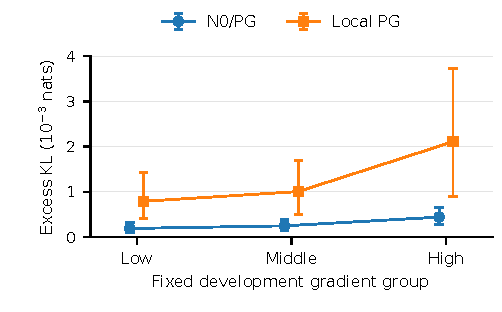
\includegraphics[width=\columnwidth]{s10_absolute_gradient.pdf}
\caption{Absolute conditional-distribution errors on the fixed 32-source development set. Points and 95\% source-bootstrap intervals use equal source weighting within each gradient group. Both errors rise with gradient; Local PG rises more. The cohort and grouping differ from the held-out marginal comparisons in Fig.~4 of the main text.}
\label{fig:absolutegradient}
\end{figure}

\begin{table*}[t]
\centering
\caption{Selected regional NLL contrasts that favor a comparator or have intervals crossing zero. N0-minus-comparator differences and pointwise 95\% source-bootstrap intervals are in $10^{-3}$ nats. The first two rows are post-hoc held-out case groups with zero fraction $z_{\mathrm{case}}\geq0.5$; the remaining rows use development candidates. Here $d$ is the Sobel magnitude of $\log(1+s)$ divided by eight, and $a$ is the four-connected zero-component size in packed pixels.}
\label{tab:adverse}
\begin{tabular}{@{}llrrrr@{}}
\toprule
Feature / bin & Comparator & Sources & Difference & \multicolumn{2}{c}{95\% interval}\\
\midrule
Case zero fraction $\geq0.5$ & Local Bayes & 30 & $+0.0020$ & $-0.0132$ & $+0.0172$\\
Case zero fraction $\geq0.5$ & Foi-qPG & 30 & $+0.0080$ & $-0.0039$ & $+0.0200$\\
Signal $0\leq s<2$ DN & N0 permuted & 28 & $+1.3432$ & $-2.3007$ & $+6.1834$\\
Signal $s\geq16$ DN & Local PG & 20 & $-1.9514$ & $-4.0343$ & $+0.2155$\\
Gradient $0\leq d<0.025$ & Local PG & 32 & $+0.0043$ & $-1.4801$ & $+1.6993$\\
Gradient $0.025\leq d<0.1$ & Local PG & 32 & $+0.1099$ & $-0.9157$ & $+1.2081$\\
Gradient $d\geq0.1$ & Local PG & 32 & $-0.8031$ & $-2.0314$ & $+0.3147$\\
Zero-component size $a\geq33$ & Local PG & 30 & $-0.5950$ & $-2.0038$ & $+0.5810$\\
Zero-component size $a\geq33$ & N0 permuted & 30 & $-0.5265$ & $-3.8384$ & $+3.0659$\\
\bottomrule
\end{tabular}
\end{table*}

\subsection{Why Pooled Curves Can Overlap}
For equally weighted distributions,
\begin{equation}
\operatorname{TV}\!\left(\frac1n\sum_iq_i,\frac1n\sum_ir_i\right)
\leq\frac1n\sum_i\operatorname{TV}(q_i,r_i).
\end{equation}
The triangle inequality gives this bound. Development mean pointwise TV is 0.01235; real pooled-PMF TVs are 0.000282 and 0.001561 on different cohorts and weights. The archived pointwise histogram retains the full diagnostic distribution. Paired scores evaluate the accuracy of the locationwise predictions.

\section{Real-Exposure and Downstream Protocols}
\subsection{Integer Alignment and Hidden References}
\begin{table}[t]
\centering
\caption{Real-data NLL and CRPS differences under tail and repeated-coordinate exclusions. N0 minus Local PG on common R/$G_1$/$G_2$ candidates; negative values favor N0. The all-event row gives the full-sample result, followed by subsets selected using the retained readouts.}
\label{tab:real_robust}
\footnotesize
\setlength{\tabcolsep}{2.2pt}
\begin{tabular}{@{}llrrr@{}}
\toprule
Frame & Included positions & $N$ & $10^3\Delta$NLL & $\Delta$CRPS (DN)\\
\midrule
4748 & All & 12,652 & $-1.342$ & $-0.01102$\\
 & $V>-128$ & 12,609 & $-1.375$ & $-0.01145$\\
 & Excl. repeat coords. & 12,650 & $-1.336$ & $-0.01098$\\
\addlinespace[2pt]
4749 & All & 19,200 & $-0.964$ & $-0.00920$\\
 & $V>-128$ & 19,121 & $-0.998$ & $-0.00927$\\
 & Excl. repeat coords. & 19,198 & $-0.945$ & $-0.00907$\\
\bottomrule
\end{tabular}
\end{table}

Real references use the fixed coordinate transformation $V=R_{\mathrm{native}}-512+n_c$, with $n_c=(2,3,3,3)$ for R/$G_1$/$G_2$/B. The original camera files remain unchanged; integer shifts preserve the quantization grid.

Independent dark-frame calibration leaves fractional residuals $(-0.437,-0.310,-0.189,+0.078)$ DN. The network and decoder retain zero inference offsets, so these residuals remain part of the real-data model mismatch.

Table~\ref{tab:tail_original} reports the fixed $-125$ DN diagnostic, distinct from the main-text $-128$ threshold. The events are nested. Section~\ref{sec:realcode} relates the extreme labels to their original decoded codes.

\begin{table}[t]
\centering
\caption{Zero-atom and tail events among all 31,852 shared real R/$G_1$/$G_2$ candidates. Expected counts sum N0 probabilities; observed counts use the retained signed labels.}
\label{tab:tail_original}
\begin{tabular}{@{}lrr@{}}
\toprule
Event & Expected count & Observed count\\
\midrule
$V=0$ & 1107.76 & 1190\\
$V\leq-1$ & 30744.24 & 30662\\
$V\leq-50$ & 1345.75 & 1065\\
$V\leq-125$ & 0.01690 & 132\\
$V\leq-305$ & $8.63\times10^{-30}$ & 13\\
\bottomrule
\end{tabular}
\end{table}

\subsection{Fixed Demosaicking Pipeline}
The fixed LibRaw 0.22.1 pipeline calls \texttt{open\_bayer(black=0)}, \texttt{unpack}, \texttt{raw2image\_ex(0)}, \texttt{pre\_interpolate}, and \texttt{ahd\_interpolate}, followed by FP32 pedestal subtraction. This bypasses ordinary black subtraction, scaling, white balance, color/gamma conversion, and denoising. Revision and patch hashes are recorded with the renderer.

Negative-pattern tests verify that below-black information reaches interpolation. In the recorded renderer validation, the fixed-source implementation reproduced all six full-frame linear RGB arrays exactly.

AHD's nonlinear decisions depend on the pedestal, as verified at $P=512$ and $P=1024$. All comparisons use $H(V+512)-512$.

\subsection{A/B/C/D Statistics}
Each real ROI is $512\times512$ Bayer pixels. Removing a 16-pixel border leaves $480\times480$ evaluated RGB pixels. A and B are fixed signed/clipped references. Each of the 32 C/D draws is demosaicked separately; spatial statistics are computed per draw before aggregation. D uses the real-data Local PG $3\times3$ window; the synthetic test uses $5\times5$.

\begin{table*}[t]
\centering
\caption{Linear camera-RGB statistics in the two preselected darkest real ROIs, before white balance or display clipping. A/B are fixed references; C/D average the spatial statistics of 32 separately demosaicked samples. Units are DN. The data contain all 12 ROIs.}
\label{tab:ahd}
\begin{tabular}{@{}llrrrrr@{}}
\toprule
Exposure & AHD input & $\mu_R$ & $\mu_G$ & $\mu_B$ & sd$(R-G)$ & sd$(B-G)$\\
\midrule
P2654748 & A: signed reference & 8.041 & 9.003 & 3.200 & 25.986 & 22.037\\
& B: clipped & 15.368 & 16.322 & 11.707 & 18.635 & 15.127\\
& C: N0 samples & 7.924 & 8.621 & 1.655 & 25.157 & 22.495\\
& D: Local PG samples & 7.933 & 8.602 & 1.642 & 25.256 & 22.587\\
P2654749 & A: signed reference & 0.423 & 0.797 & $-0.225$ & 23.584 & 20.529\\
& B: clipped & 10.089 & 10.287 & 9.146 & 15.243 & 12.712\\
& C: N0 samples & 0.231 & 0.246 & $-1.871$ & 22.813 & 20.860\\
& D: Local PG samples & 0.352 & 0.352 & $-1.812$ & 22.799 & 20.861\\
\bottomrule
\end{tabular}
\end{table*}

Table~\ref{tab:ahd} reports the two preselected darkest ROIs. Each draw contributes its own spatial mean and standard deviation; intervals describe variation across draws. Spatial standard deviations include scene texture and demosaicking correlation.



\subsection{Processing-Order Illustration}
\href{visual_en.pdf}{Supplementary Visual A} shows the P2654749 crop at $(0,1500)$: $1000\times1000$ Bayer pixels, full-frame AHD, and fourfold area reduction to $250\times250$ pixels. The labeled routes differ in RAW/RGB clipping order and share exposure and display transforms.

\subsection{Fixed Clean-Reference Color Endpoint}\label{sec:cleanendpoint}
This development experiment followed the earlier analyses, with its protocol fixed before the color scores were computed. The protocol specifies the renderer and error metrics, with no preset perceptual-effect threshold. Eight geometrically complete natural crops were selected from the 32-source development set without using endpoint scores; four procedural templates were evaluated separately. Each scene generated 16 independent PG sensor realizations and two conditional draws per estimator and realization. The renderer used integer AHD with pedestal 512, fourfold signed-domain integration, fixed white balance and color matrix, and one clean-reference exposure per scene. After excluding the score border, the eight blocks with lowest clean-reference luminance formed the evaluation region. We measured squared block-mean $(R-G,B-G)$ error in exposure-scaled linear display RGB against clean-$Q$-AHD, where $Q(s)=\lfloor s+0.5\rfloor$. Conditional means were quantized with the same $Q$ before AHD. We scored each draw separately, averaged within sensor realization, and then weighted the eight natural sources equally.



N0 sampling reduces dark-color error by $0.003139$ relative to Local PG (paired source-bootstrap 95\% interval $[-0.006136,-0.000843]$), with lower error on all eight natural sources. The two largest reductions contribute 67.9\% of the total improvement. Quantized-mean completion reduces the N0 color error by a further 16.5\% relative to sampling. For clean-RAW MSE, N0 sampling instead exceeds Local PG by $2.062$ DN$^2$ (95\% source interval $[0.713,3.834]$); only one of eight source differences favors N0. The signed arm uses the uncensored readout of each of the 16 sensor realizations, with clean-$Q$-AHD as a separate color reference. Its paired color-error difference from N0 spans zero. All 12 sources, secondary scores, and per-draw records are supplied; the eight-source values are also collected in \texttt{evidence/clean\_color/}\allowbreak\texttt{PER\_SOURCE.csv}.

\section{Numerical and Reproduction Records}
Inference uses a 256-pixel core and a 192-pixel halo in packed CFA coordinates. Core and halo sizes are multiples of 16, preserving the encoder phase. Measurements and validity masks are zero-padded to a multiple of 16; tiles are clipped at the image boundary, and only their core predictions are retained. The released implementation specifies this procedure in \texttt{inference/tiling.py}. Sampling uses absolute pixel coordinates as described in Section~III. The accompanying records retain decoder identities and reproduction tolerances.

\section{Additional Development Controls}\label{sec:v3}
The following post-hoc controls use development data and supplement the registered independent test.

\subsection{Joint-CFA Local Development Comparator}
Joint-CFA local Bayes uses 256 equally weighted four-phase signal templates from 128 training scenes, with two templates per scene. A packed $5\times5$ likelihood includes all valid four-phase observations and counts each censoring event once. Prediction mixes the corresponding conditional integer PG laws. N0 and both local estimators are evaluated at the same 32,462 positions from 32 development sources.

\begin{table}[t]
\centering
\caption{Post-hoc development comparison on 32 fixed sources. CFA means are computed within source, followed by equal source weighting.}
\label{tab:joint}
\scriptsize
\setlength{\tabcolsep}{3pt}
\begin{tabular}{@{}lrrr@{}}
\toprule
Method & Excess KL & NLL & CRPS\\
& (nats) & (nats) & (DN)\\
\midrule
N0/PG & 0.000376673 & 3.911227506 & 8.103882756\\
Joint-CFA local Bayes & 0.001790969 & 3.912282251 & 8.112198163\\
Same-CFA Local PG & 0.001952344 & 3.912362493 & 8.112870272\\
\bottomrule
\end{tabular}
\end{table}

N0 minus Joint-CFA differences, with 95\% source-bootstrap intervals, are: KL $-0.00141430$ [$-0.00296235,-0.00031761$]; NLL $-0.00105475$ [$-0.00215630,-0.00029750$]; and CRPS $-0.00831541$ DN [$-0.01755261,-0.00217521$]. Joint-CFA minus Local PG NLL and CRPS intervals cross zero.



\begin{figure*}[t]
\centering
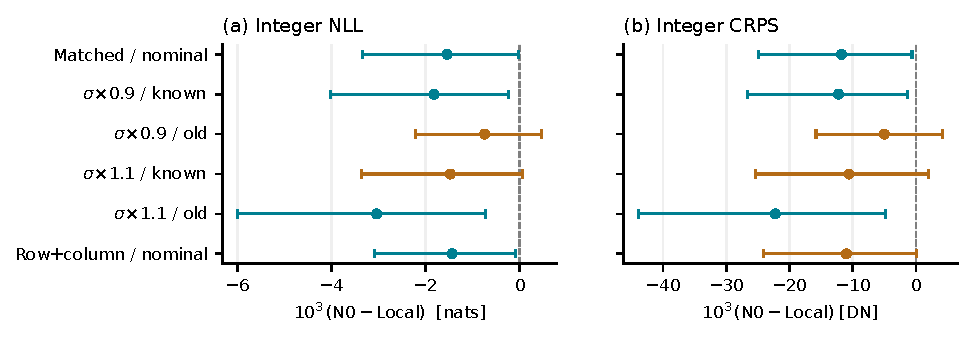
\includegraphics[width=\textwidth]{f09_paired_stress.pdf}
\caption{Paired calibration and correlation tests on 32 development sources. Each setting uses 8,192 central zero candidates shared by both methods. Points show mean differences averaged first over CFA phases and then over sources, with 95\% source-bootstrap intervals; negative values favor N0. ``Known'' supplies the changed profile to both estimators and their decoders; ``old'' retains the original calibration. Row/column offsets are unobserved. Orange intervals cross zero.}
\label{fig:pairedstress}
\end{figure*}

\subsection{Runtime and Resource Table}
\begin{table}[tbp]
\centering
\caption{In-memory implementation cost. Decoding, initialization, and file output are excluded; backends and warm-up differ as specified in the text.}
\label{tab:runtime}
\footnotesize
\begin{tabular}{@{}lrr@{}}
\toprule
Metric & N0/PG & Local PG $3\times3$\\
\midrule
128 packed median (s) & 0.2074 & 0.7329\\
24MP median of 3 (s) & 27.3901 & 205.1503\\
24MP range (s) & 25.1087--27.9992 & 194.3892--219.9394\\
CUDA allocated (MiB) & 750.69 & 94.84\\
CUDA reserved (MiB) & 1112.00 & 254.00\\
\bottomrule
\end{tabular}
\end{table}

Timings use an RTX 3090 Ti, Python 3.10, PyTorch 2.6/CUDA 12.4, two CPU threads, and synchronized GPU stages. The 24MP input has 2,637,992 zeros. Patches use 10 warmups/30 runs; N0 full-frame uses 10 warmups, while Local PG combines one pilot/two later runs. N0 uses FP32 network/GPU LUT; Local uses FP64 GPU likelihood/CPU LUT; both sample on CPU. Full timings are archived.

Local PG core/halo is 128/1. At 32 checked positions, signal error is below $3.05\times10^{-12}$ DN and LUT PMFs match. The checked tile MLEs remain at least 179.14 DN below the grid limits.

\subsection{Paired Calibration and Correlation Probes}
N0 and same-CFA $5\times5$ Local PG use the same generated inputs from 32 development sources: a 128-pixel packed context, central 64-pixel region, and at most 64 zeros per phase. Scores are averaged over CFA phases and then sources. The paired 95\% intervals use 10,000 source resamples. Candidates are shared between methods within each setting and can differ between settings.

At read-noise factors 0.9/1.1, both methods receive either the true new profile or the old profile; known-profile network constants extrapolate beyond training. Gaussian row/column offsets each have 5 DN standard deviation and are withheld from both methods. That condition reports no oracle-KL. Integer scoring resolves the PG tail.

Fig.~\ref{fig:pairedstress} reports all conditions. Old calibration at $0.9\sigma$ gives NLL $-0.000746$ nats, interval $[-0.002214,0.000462]$; known $1.1\sigma$ also has inconclusive contrasts. Row/column offsets give NLL $-0.001439$, $[-0.003090,-0.000090]$, while the CRPS interval crosses zero. The accompanying data include full scores, profile probes, and rare-tail tests.

\subsection{Real-Code Event Scope}\label{sec:realcode}
All 31,852 primary real candidates remain scored. The nested $-128/-256/-305$ thresholds contain 122/21/13 events. The deepest 13 decode to native 79--202 and aligned $-430$ to $-307$ DN. Two coordinates repeat below $-128$, one below $-305$; the full frames separately contain 18/25 native zeros. The ten dark frames supply calibration. Although the deepest events contribute 0.03917/0.04525 nats to absolute N0 NLL, they change the paired difference by only $+0.0000040/-0.0000083$. Removing $V\leq-128$ leaves NLL differences of $-0.001375/-0.000998$ (Supplementary Table~\ref{tab:real_robust}).

N0 has lower NLL in 7/12 fixed ROIs. Symmetric 1\% winsorization gives differences of $-0.001269/-0.001082$, compared with $-0.001342/-0.000964$ for all events. B-phase diagnostic N0/Local NLL is 3.807768/3.810883 and 3.857925/3.859954 in the two exposures, using the shared R/$G_1$ noise calibration. The data retain all ROI/CFA contributions.

\end{document}
